\chapter{State of the art}\label{chapter:stateofheart}
\nomenclature{CPU}{Central Processing Unit}
\nomenclature{FPGA}{Field Programmable Gate Array}
\nomenclature{SIFT}{Scale-Invariant Feature transform}
\nomenclature{CV}{Computer Vision}
\nomenclature{MLS}{Moving Least Squares}

One of the first car applied camera-based ADAS(Advanced Driving Assistance System) was the rear camera. This system consists on a wide-angle camera on the vehicle rear and a driver display. This system can be found in many large vehicles as a parking guidance, as long as the driver does not have any direct visibility due to the interior mirror absence.

One of this system evaluations is the 360\degree~vision system. This system includes several cameras --usually from 3 to 6-- located around the vehicle. The system does not only show the image from the cameras, but also merges them in one virtual top-view image. The first 360\degree~vision systems for cars were available only on high-end vehicles as a luxury accessory. However, nowadays many mid-end vehicles also offer this feature \cite{nissan}.

In this section the most relevant 360\degree~commercial systems are briefly described. As long as the technical details about this systems is not available, the description will focus on technical aspects extracted from promotional and non-official reviews.

Besides the commercial systems this chapter also describes the algorithms used in overhead image stitching. This chapter second part contains the main algorithms description, either those specific for bird's eye view or those generic stitching algorithms relevant on this work.

\section{Commercial systems}\label{sec:commercial_state}
Currently there are several manufacturers that offers an 360\degree~view systems. Most of this systems have similar features, such as the number of cameras or the available viewpoints available. In this section the most relevant ones will be described, focusing on the main features and the relevant technical details. 

\subsection{Nissan: Around View Monitor}\label{ssec:nissan_commerc_state}
The system presented by Nissan in their \emph{Around View Monitor} consists on four cameras located around the vehicle --one at the front, one at each rearview and one at the rear. The captured images are  deformed to match an specific ground pattern\footnote{\cite{calibration} shows the calibration process for a car 360\degree~vision system}. The four deformed images are shown on a single canvas. In some working modes, in this canvas are also overlapped lines showing the vehicle path of the vehicle according to the steering wheel rotation and current speed. \cite{totnissan}

As it can be seen in Figure~\ref{fig:nissan-state}, the four images are undistorted --the effects of the fisheye lens are compensated-- and aligned to a common ground. However, this screenshot shows that the front camera presents a +10cm misalignment with the lateral cameras. However, this misalignment is acceptable in this application because the four images are not merged. In the application presented in this project, however, the four images are merged in an unique image --not four fragments. Thus, this misalignment level cannot be admitted. 

\begin{figure}[h]
\center
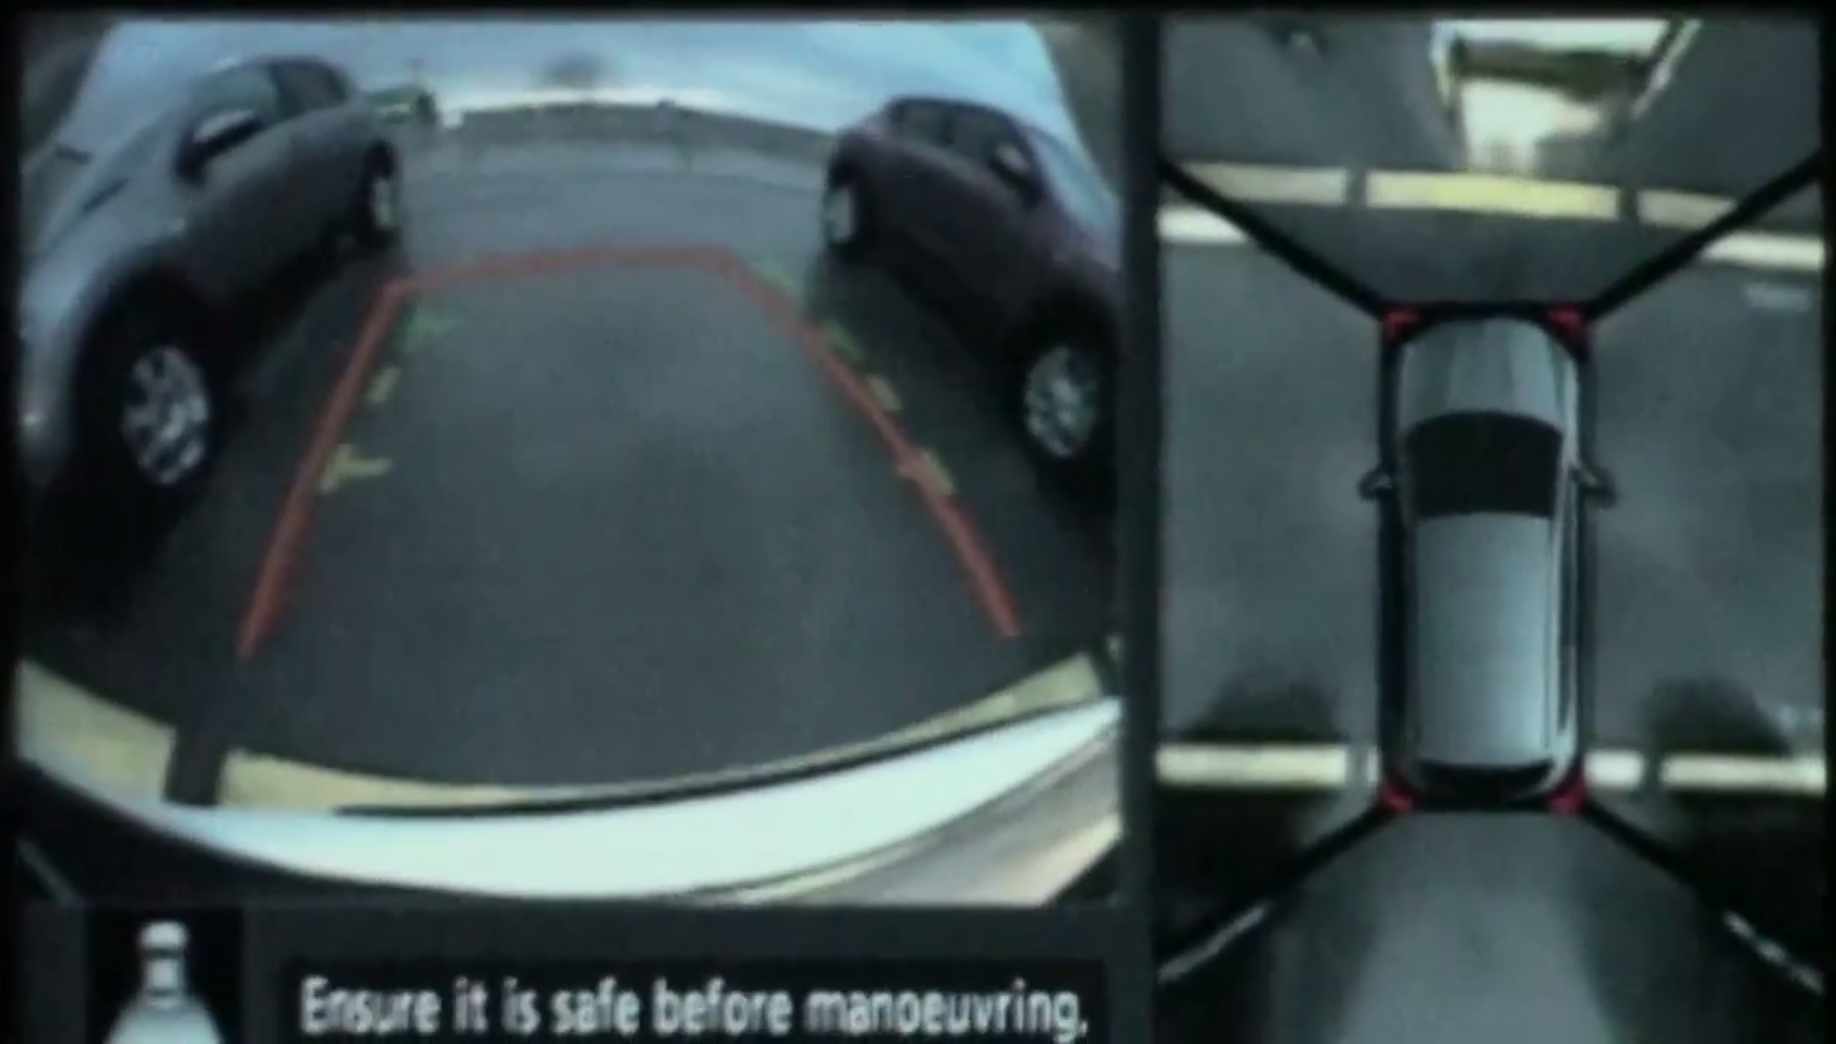
\includegraphics[width=0.58\textwidth]{images/nissan-state}
		\caption{Around View Monitor system screenshot on a Nissan Qashqai \cite{videonissan}}
		\label{fig:nissan-state}
\end{figure}

This system was first installed in Nissan Elgrand --a luxury vehicle--, but now it can be found in mid-end vehicle as Nissan Note.This system is offered by other brands, such as BMW (Surround view System) or Infinity (Around View Monitor). There are also manufacturers specialized on vehicle accessories that also offers this system, such as Alpine (HCE series). \cite{infiniti} \cite{calibration}

\subsection{Audi: 360\degree~View Camera}\label{ssec:audi_commerc_state}
Audi offers a similar 360\degree{} vision system: the \emph{360\degree~View Camera}. This system has the same camera setup than Nissan \emph{Around view monitor}. However, in this case the four images are blended into one image. A smooth transition is performed on the overlapping areas between cameras to make a single camera effect. \cite{videoaudi}

As it can be seen in Figure~\ref{fig:audi-state}, the four cameras are effectively merged in one single image, but there are still misalignment between cameras. On the  vehicle front right side it cat be seen that a ground line disappears in the transitions between the two cameras. Moreover, on the front left side the white car can only be seen partially.  

\begin{figure}[h]
\center
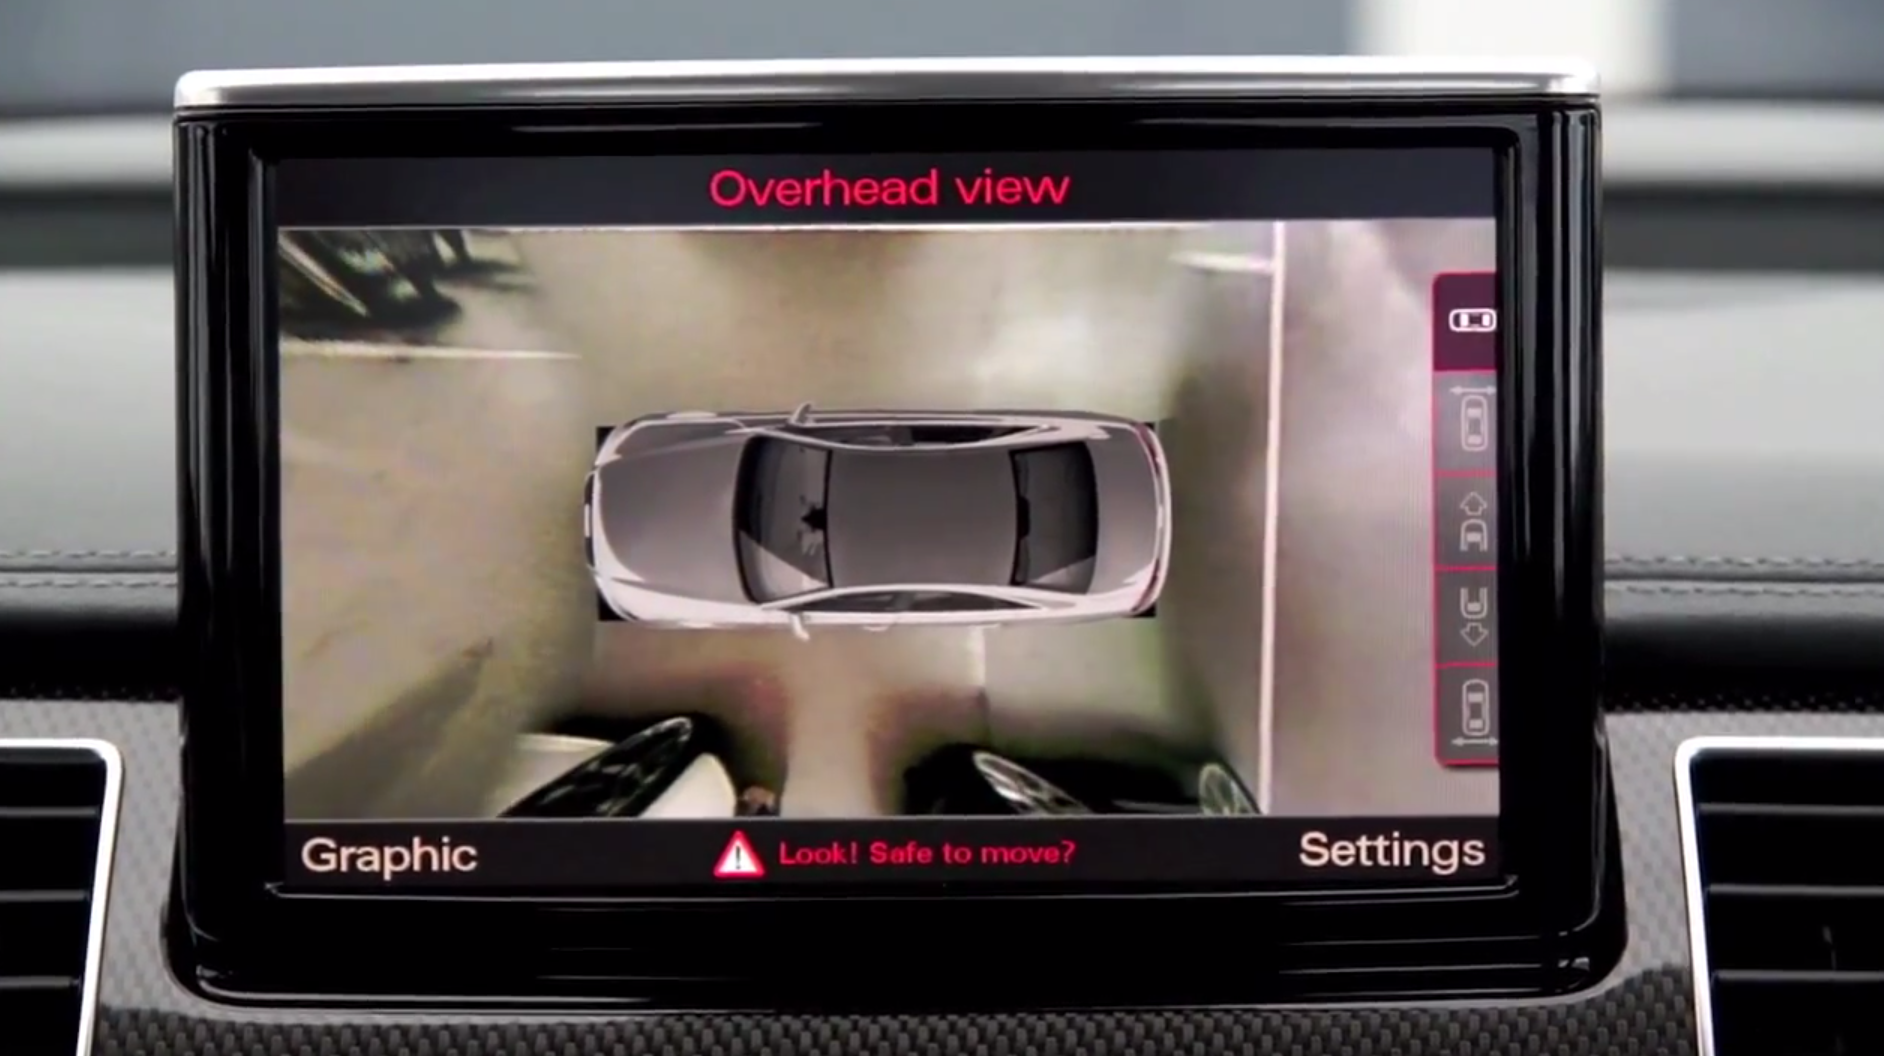
\includegraphics[width=0.58\textwidth]{images/audi-state}
		\caption{360\degree~View Camera on an Audi S8 screenshot \cite{videoaudi}}
		\label{fig:audi-state}
\end{figure}

This project will focus on solving the image misalignment only on ground level, so the ghost image of the white vehicle will still be present with the approaches presented. However, the misalignment --or disappearance-- on ground-level lines is an aspect to be improved on this project.

A similar system can be found on some VolksVagen models --such as Touareg--. In this system, however, the overlapped area is marked with thin delimiter lines. \cite{touareg}

\subsection{Fujitsu: Multi-Angle Vision}
The \emph{Multi-Angle Vision} system by Fujitsu presents a different approach than Nissan and Audi ones. Instead of wrapping the image on a planar surface to obtain an overhead view, this system wraps the four images on a single hemisphere centred on the vehicle, as it can be seen in Figure~\ref{fig:fujitsu-mesh-state}. \cite{fujitsu}

\begin{figure}[h]
	\centering
	\begin{subfigure}[b]{0.48\textwidth}
		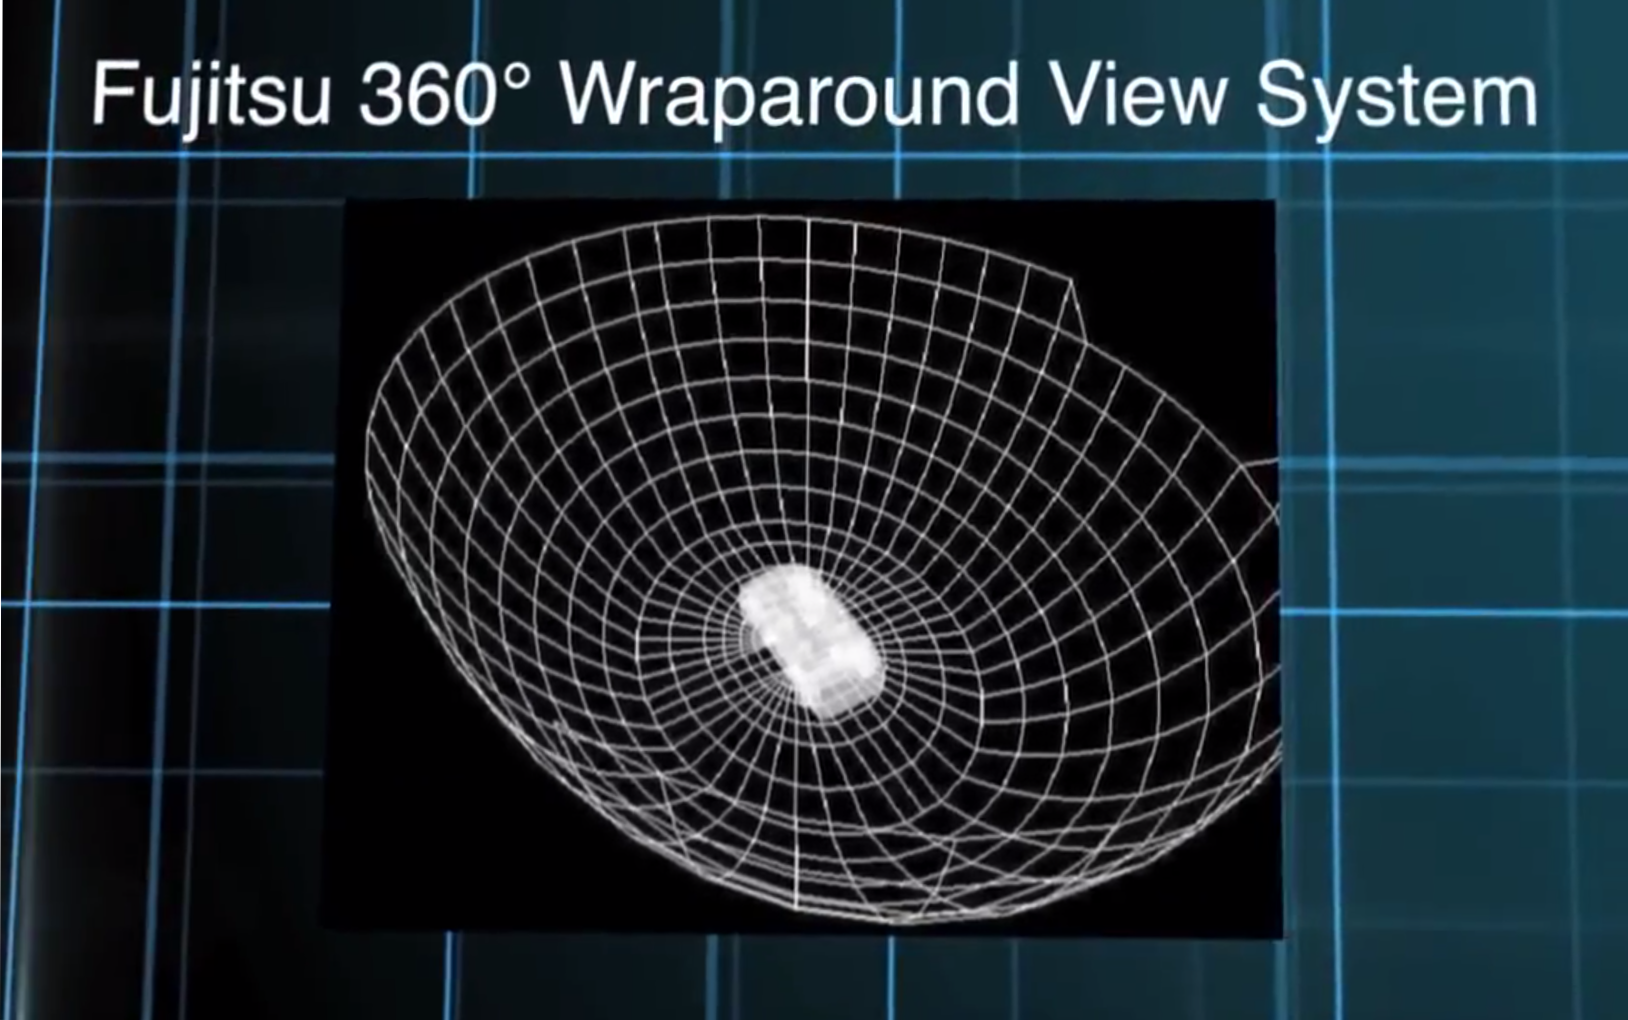
\includegraphics[width=\textwidth]{images/fujitsu-mesh-state}
		\caption{Synthetic mesh where the four images are projected}
		\label{fig:fujitsu-mesh-state}
	\end{subfigure}
	\hspace{0.2cm}
	\begin{subfigure}[b]{0.443\textwidth}
		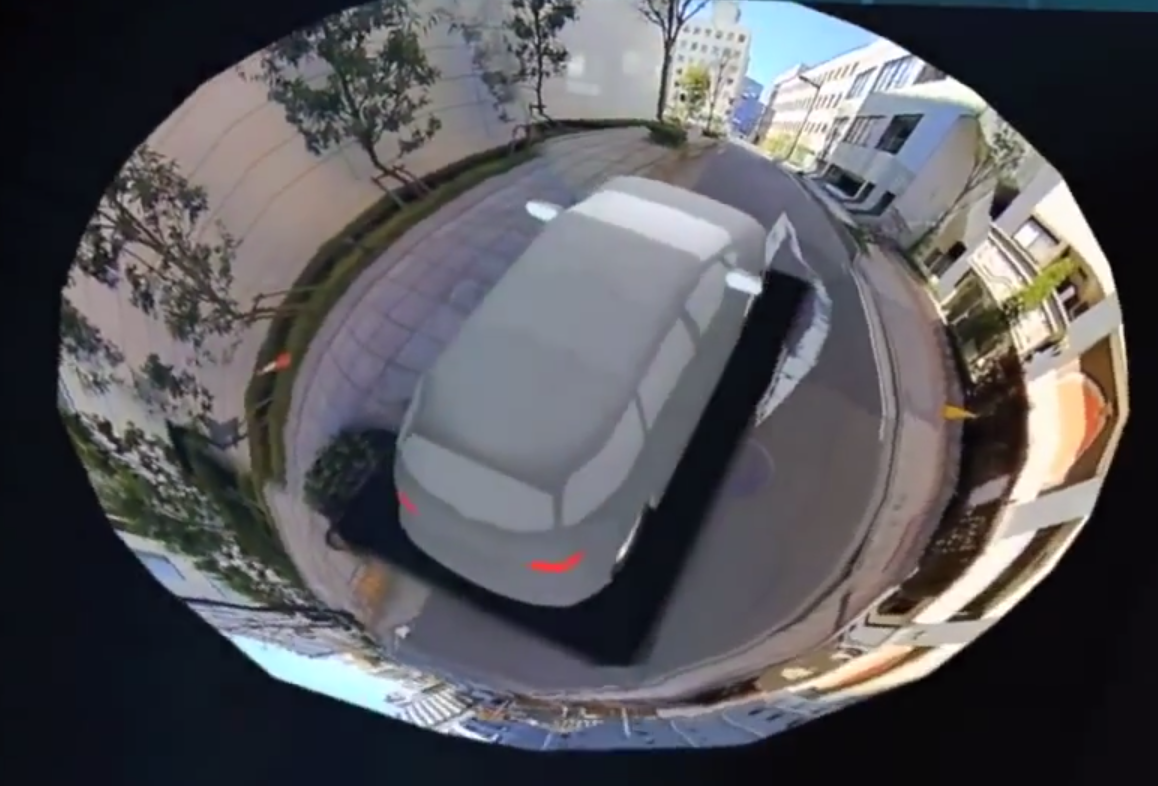
\includegraphics[width=\textwidth]{images/fujitsu-360-state}
		\caption{One viewpoint from the images projected on the mesh}
		\label{fig:fujitsu-360-state}
	\end{subfigure}
	\caption{Mesh and output image of Fujitsu Multi-Angle Vision  \cite{fujitsu}}
	\label{fig:fujitsu-state}
\end{figure}

This powerful system allows the user to select the viewpoint, and also minimizes the ghost effect on elements above the ground plane. This system can offer many viewpoints to the driver by rendering the mesh from any viewpoint. If it is rendered from above, the image is a deformed bird eye view, with and higher viewed area than the previous systems. The usage of many viewpoints allow the driver to see in more detail different surroundings points --lateral views of the road, frontal view on an intersection of streets, rear view when parking, etc. However, this system has minor drawbacks. First of all,there are still minor errors on the transitions between images that seem not easy to solve. Another minor drawback is that the mesh system makes more difficult to draw the vehicle path lines on the image, as seen in Nissan approach.

Although a modification based on this system may offer high quality results in this project, this approach is not explored in this TFG. The lack of information about the procedure used and the probably high computational cost left this research path to a future iteration of the project.

\subsection{Land Rover: Surround Camera System}\label{ssec:land_commerc_state}
Land Rover offers a different system than the ones stated before. Instead of using four cameras, the Surround Camera System 	uses five cameras: two on the front --left and right-- two on the sides --left and right-- and one on the rear. However, this system does not perform any stitching. Instead, the five images are shown in a grid as seen in Figure~\ref{fig:landrover-state}.  \cite{landrover}

\begin{figure}[h]
\center
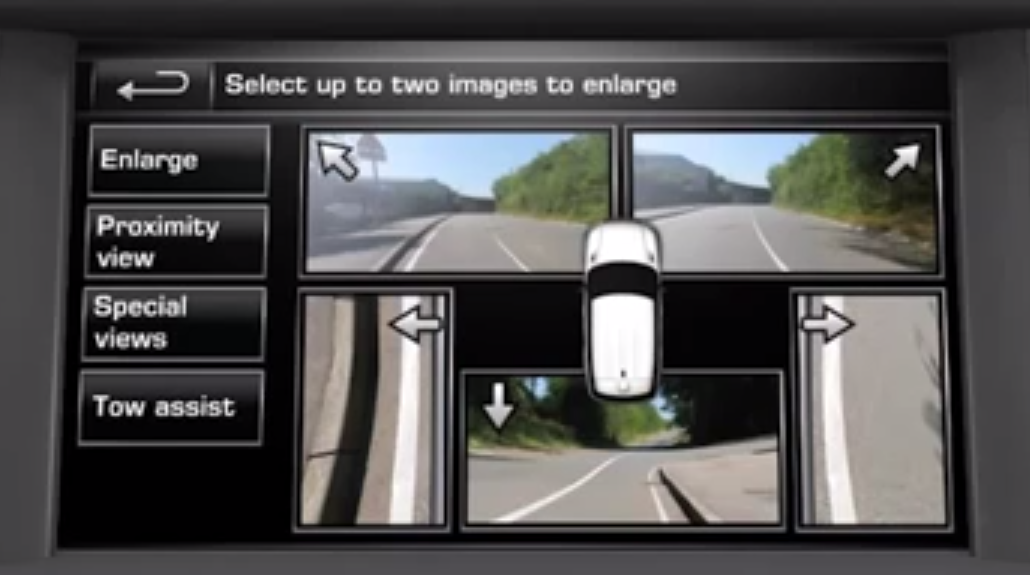
\includegraphics[width=0.6\textwidth]{images/landrover-state}
		\caption{Screenshot of the Surround Camera System on Land Rover \cite{videolandrover}}
		\label{fig:landrover-state}
\end{figure}

Although this system can offer a complete view around the vehicle using more cameras, this is not included in this project goals. Placing the cameras on the corners rather than on the sides, however, is an option for future iterations on the Arcol project.

\section{Technical information}
There are two main sources regarding 360\degree~vision stitching system: general information about image stitching --mainly form panorama creation-- and specific information about bird's eye systems for passenger vehicles.

Although panorama stitching and bird's eye stitching are different systems, they share a common pipeline. This can be summed up as shown in Figure~\ref{fig:simple-pipeline}. \cite{opencvpipeline}

\begin{figure}[h]
\center
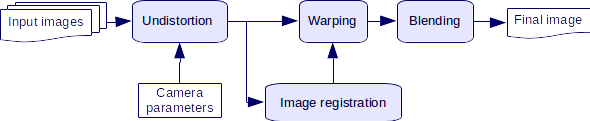
\includegraphics[width=0.9\textwidth]{images/simple-pipeline}
		\caption{Simple pipeline for image stitching}
		\label{fig:simple-pipeline}
\end{figure}

As it can be seen, the stitching process is divided in main 4 blocks: undistortion, image registration, warping and blending. 

The undistortion step consists on removing all the lens effect, mainly modelled with radial and tangential distortion. Although this step is outside the scope of this project, the quality of the undistortion algorithm will affect the next steps. The resulting image resulting of this step should only present perspective deformation.

Image registration consists on detecting a points set on a image and assign them either to another image or to a common ground plane. In panorama image stitching the different key points are related from one image to another, but in 360\degree{} vision systems the key points are related to the ground calibration pattern view. This project will only perform a manual key point registration, leaving the automatic process to a future iteration.

Warping is the technique to deform the undistorted image to match a set of defined key points. This part will be fully developed in this project.

Once the images are deformed, in the blending step the merging parameters and techniques are applied. Although this step is outside this project scope, basic techniques will be developed to obtain a final stitched image.

\subsection{Image registration}
To define the key points or features on the image two main techniques are used: automatic feature detection and pattern-based features.

\subsubsection{Automatic registration}
Automatic feature detection is used when a custom pattern cannot be defined. This is the case of panorama stitching, where the images to be stitched are not previously known and cannot be calibrated. In this case, the image are analyzed to detect relevant points.

Once the automatic features are detected the next step is to perform a two-by-two matching between the features of the different images. As long as the different images are not completely overlapped, only a feature subset from each image will have a correspondence to the other image. Moreover, there can be outliers --correspondences between images that are wrongly established-- and valid  features that have not been detected.

If the automatic feature detection  has been done correctly and there is enough overlapping area, the amount of  correctly detected correspondences will be large enough to discard outliers and establish a pattern matching. Then, the next step, warping, can be performed. Figure~\ref{fig:autocorresp} shows an example image with features correctly matched between two viewpoints.
\begin{figure}[h]
\centering
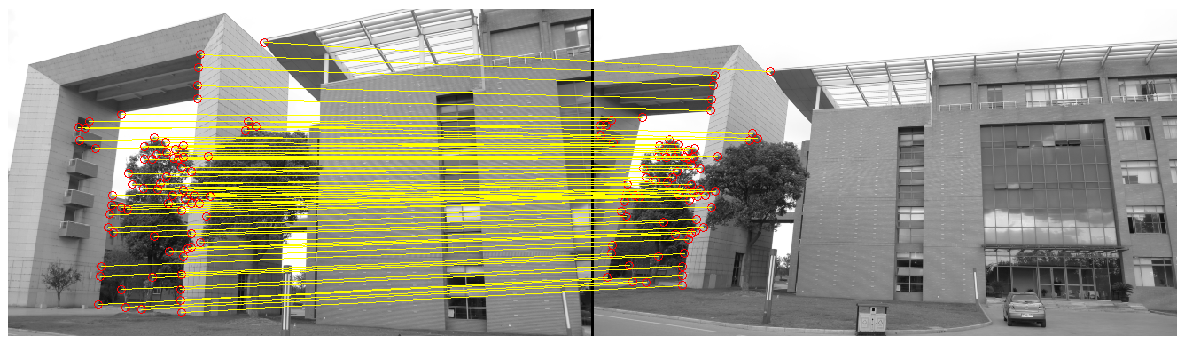
\includegraphics[width=\textwidth]{images/correspondence}
\caption{Automatic detected matching correspondences between two images  \cite{tongji}}
\label{fig:autocorresp}
\end{figure}

This approach main drawback is that relies on the image information. If the image does not have significant points --contrast changes, distinguishable textures, enough overlapping area, etc.-- the stitching process will not obtain good results. However, if the image has enough information the stitching obtained can be very precise.

In the case of 360\degree{} vision systems, as it can be seen in the commercial systems, the information and precision in the camera images is significantly low. In addition, the overlapping areas between two cameras is very low or, with fisheye cameras, the distortion on this area is very high. This two factors motivate a pattern-based feature detection system usage.

\subsubsection{Custom pattern registration}
A completely different approach for image registration is the use of a ground pattern. In this case, the pattern is placed in a specific position to perform the calibration step. Then, all the cameras whose images are going  to be stitched capture a frame showing the pattern in its position and the pattern is detected. 

The key points set are obtained from the detection are matched with the actual pattern position. Using this method each image deformation parameters are estimated. In running time, the deformation previously computed is applied to all the images. The patterns used in this project can be seen in Figure~\ref{fig:patterns}.
\begin{figure}
\center
	\begin{subfigure}[b]{0.48\textwidth}
		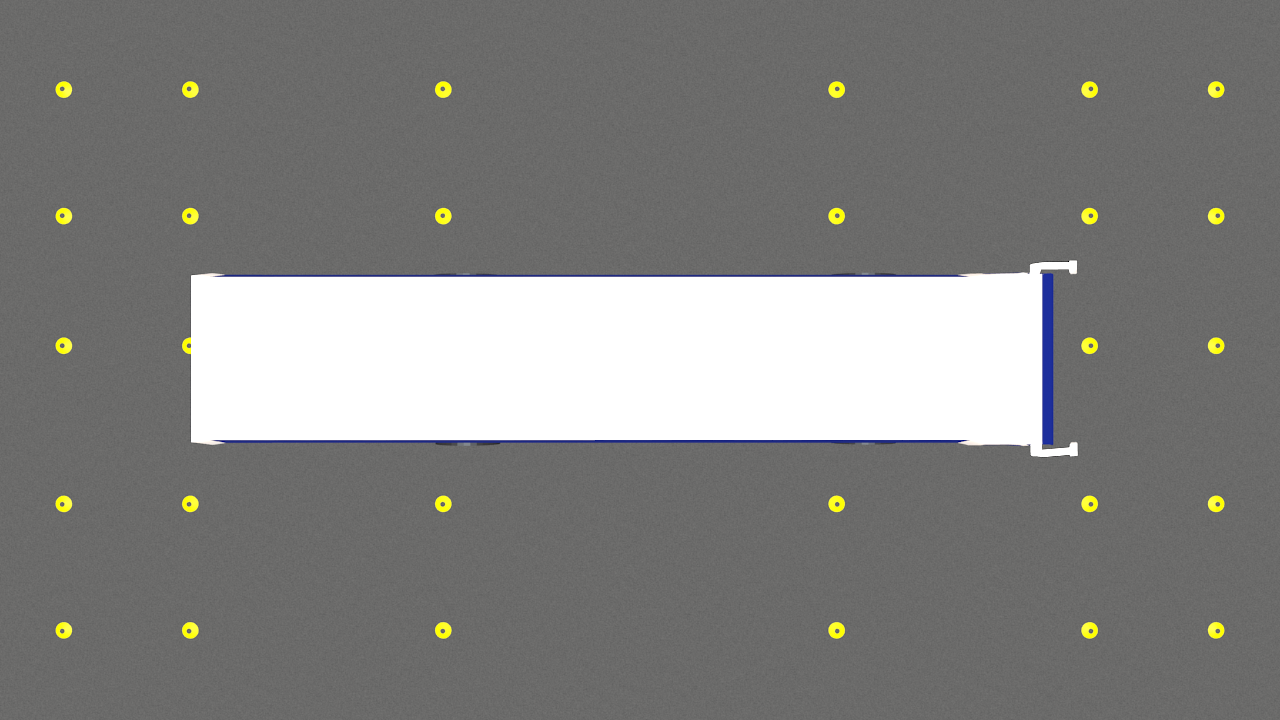
\includegraphics[scale=0.15]{images/pattern1}
		\caption{Cone pattern.}
	\end{subfigure}
	\begin{subfigure}[b]{0.48\textwidth}
		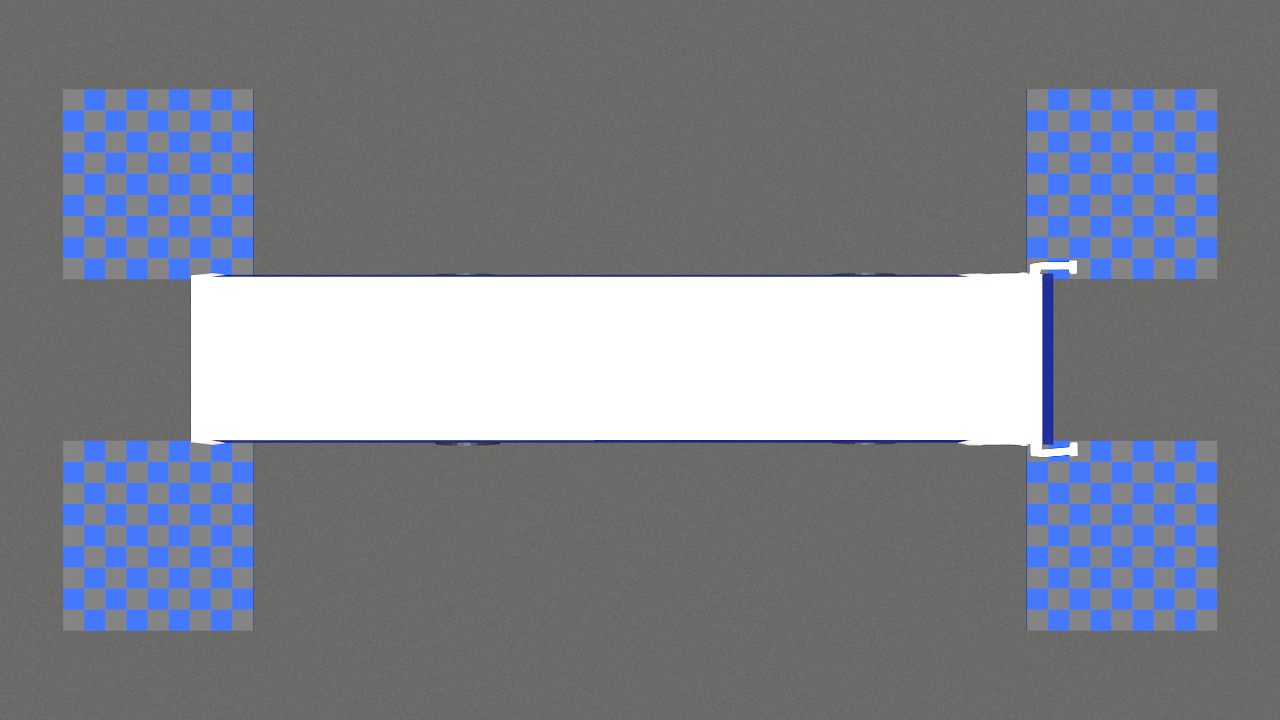
\includegraphics[scale=0.15]{images/pattern2}
		\caption{Chessboard pattern.}
	\end{subfigure}
	\caption{Virtual view of the patterns used in this project.}
	\label{fig:patterns}
\end{figure}
  
This approach is widely used in 360\degree vision systems. In this case, the cameras are not moved during the different captures, as they are solidly attached to the vehicle and thus a previously calibration step can be done. Thus, a previous calibration step can be done.

The usual configuration is done by putting a pattern on the floor -for simplicity- and capture the image seen from each camera. This pattern can be either centred on the image -the area with better vision- or in the overlapping area between images. 

This method establishes a relationship between the scene 3D points and the ground. This allows to project the image in a canvas where the reference points can be defined without ambiguity. 

For the reasons stated before --non-image dependency, custom canvas, offline calibration step--  this approach will be used in this stitching application, rather than using automatic registration.


\subsection{Warping}
The warping algorithms deform the image following a constraints set. In this stitching context, this constraints set can be summed up as a point pairs set, ones referring to points in the original image and ones referring to points on the canvas.

There are several techniques to deform the image following this constraints. Depending on the method complexity degree the procedure aggressiveness , the resulting image presents a different error degree on the key points.

In this specific context, the point pairs set between the image and canvas is from 10 to 32 points, whereas in panoramic image stitching, for example, the key points set can be from hundreds. The small key points set used makes that the most aggressive algorithms, although providing a lower error on the key points, produce an unacceptable deformation on the image.

The most common algorithm and less aggressive algorithm for image deformation is \emph{homography}.  To provide a better fitting on the key points two different algorithms --with their variants-- can be found: \emph{Minimum Least Squares} and \emph{Polynomial deformation}.

\subsubsection{Homography}\label{sec:statehomo}
Homography is the most common procedure to deform an image and perform an stitching. It consists on assigning to each point of the destination image $D[k,l]$ a point of the origin image $O[m,n]$. Thus, the deformation is done following the equation that can be described with the matrix $H$ --size $3\times3$ homography matrix--.
\begin{align}
D[m',n']=I[m,n]\end{align}\begin{align}
\begin{bmatrix}
t_i m' \\
t_i n' \\
t_i
\end{bmatrix}=
\begin{bmatrix}
h_{11} & h_{12} & h_{13} \\
h_{21} & h_{22} & h_{23} \\
h_{31} & h_{32} & h_{33}
\end{bmatrix}
\begin{bmatrix}
m \\
n \\
1
\end{bmatrix}
\end{align}
This projective deformation is the affine transformations contstraintless form. This transformations include rotation, translation and scaling. Each one of this deformations can be described with an $H$ matrix with specific parameters \cite{szeliski}. This transformation is done on the projective space using homogeneous coordinates $[m,n,1]$. An additional coordinate ($t_i$) results from the $H \cdot x_{in}$ operation. Therefore, the resulting coordinates had to be normalized with this $t_i$ factor in the back conversion to the Cartesian coordinates $[m,n]$

To compute the $H$ matrix, the OpenCV\footnote{OpenCV is an open-source library used for Computer Vision.} routine \emph{findHomography} is used. The main parameters, options an algorithms used by its function are described in Section~\ref{sec:homo}.

\subsubsection{Moving Least Squares}\label{sec:statemls}
Moving least squares method, as opposed to the homography method, does not make a global deformation in the whole image. Instead of that, this algorithm makes a local deformation near each key point.\cite{mls}

This algorithm is mesh-based. A mesh is an image subdivision in small squared \emph{subimages}. Each division contains typically from 3 to 30 pixels by side. The deformation applied by the method is not done individually on each pixel. Instead, each mesh vertex is deformed, and the pixels inside each mesh square are deformed accordingly to the mesh deformation. Figure~\ref{fig:mls} shows the test shape deformation using three different MLS methods.
\begin{figure}[h]
\centering
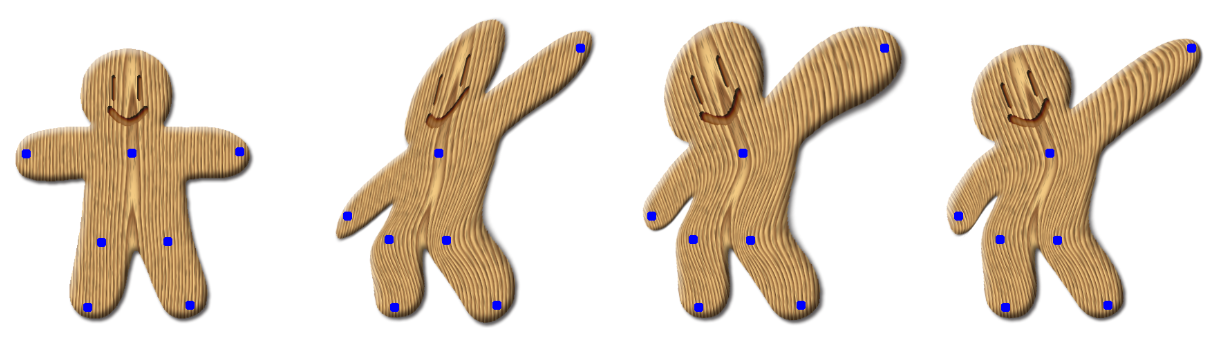
\includegraphics[width=\textwidth]{images/mls}
\caption{Test shape deformation using MLS techniques. From left to right: original image with control points, affine MLS, similarity MLS and rigid MLS.}
\label{fig:mls}
\end{figure}


\subsubsection{Polynomial deformation}\label{sec:statepoly}
Polynomial deformation --or polynomial distortion-- \cite{imagemagick} is a mapping-based deformation system. A mapping, also used in the CV (Computer Vision) algorithms, is matrix with the output image size, where each pixel contains a coordinate referring to an input image point. To obtain the value of each $I_{out}[m,n]$ output pixel, the mapping table is used as a look up table. The position $[m,n]$ of the mapping matrix will contain a coordinate $[m',n']$ from the input image. This coordinate corresponds to the $[m,n]$ output image pixel.
\begin{align}
M[m,n]=[m',n'] &: \quad \left[ \begin{aligned}
    m&=0\cdots M_{out},&  n&=0\cdots N_{out} \\
    m'&=0\cdots M_{in},&  n'&=0\cdots N_{in}
  \end{aligned}\right]\\
I_{out}[m,n] &: m=0\cdots M_{out},  n=0\cdots N_{out}\\
I_{in}[m',n'] &: m'=0\cdots M_{in},  n'=0\cdots N_{in}
\end{align}
\begin{align}
I_{out}[m,n]=I_{in}\left[M[m,n]\right]
\end{align}

This approach will be fully described in Chapter~\ref{chapter:methodology}, as it will be an important part of the final stitching algorithm.

Imagemagick is an image deformation tools complete set\cite{imagemagick} that provides an environment to perform almost any kind of image processing. One of them is the \emph{polynomial distortion}.

This deformation type assigns each deformation matrix value following a polynomial deformation. As example, Table~\ref{table:deformpoly} shows the polynomials from order 1 to 2 and its degrees of freedom. $X_s,Y_s$ corresponds to the point on the source image, whereas $X_d,Y_d$ corresponds to the points on the destination image.

\begin{table}[H]
\center
\begin{tabular}{ m{1cm} M{0.7\textwidth} m{1cm} }\hline
Order & Polynomial & DoF\\\hline\hline
\vspace{1em}1 & $X_d=C_{2x}\cdot X_s + C_{1x}\cdot Y_s + C_0x$ \newline
    $Y_d=C_{2y}\cdot X_s + C_{1y}\cdot Y_s + C_0y$ \vspace{0.2em}& \vspace{1em}6 \\ \hline
\vspace{1em}1.5 & $X_d=C_{3x}\cdot X_s \cdot Y_s + C_{2x}\cdot X_s + C_{1x}\cdot Y_s + C_0x$ \newline
    $Y_d=C_{3y}\cdot X_s \cdot Y_s +C_{2y}\cdot X_s + C_{1y}\cdot Y_s + C_0y$  \vspace{0.2em}& \vspace{1em}8 \\ \hline
\vspace{1em}2  &$X_d = C_{5x} \cdot X_s^2 + C_{4x} \cdot X_s\cdot Y_s + C_{3x}\cdot Y_s^2 + C_{2x}\cdot X_s + C_{1x}\cdot Y_s + C_{0x}  $ \newline
    $Y_d=C_{5y}\cdot X_s^2 + C_{4y}\cdot X_s\cdot Y_s + C_{3y}\cdot Y_s^2 + C_{2y}\cdot X_s + C_{1y}\cdot Y_s + C_{0y}$& \vspace{1em}10 \\\hline
\hline\end{tabular}
\caption{Deformation polynomials of the \emph{imagemagick} toolbox. Note: DoF=Degrees of Freedom.}
\label{table:deformpoly}
\end{table}
\vspace{-1.4em}
The deformation equations $C$ parameters of the deformation equations can be estimated using a points set $[m,n]\longmapsto[m',n']$. This points are the detected points coordinates on the image and the desired placement on the output image. In order to be computed, each pair $C_x, C_y$ needs at least one coordinates pair $[m,n]\longmapsto[m',n']$.

\subsection{Blending}
\emph{Blending} consists on merging two or more images into a single image. Although this procedure is outside the scope of this project, it is necessary to apply a blending algorithm to obtain visible results. Therefore, several simple and non-definitive procedures will be applied .

There are several algorithms to perform the blending step. The most widely used are the following:
\begin{description}[font=\normalfont\textsl]
\item[50\% blending.] This is the simplest procedure. It consists on merging each overlapped pixel in a 50\% merging from the two images pixels. This system offers poor results. It is only used to detect errors on the overlapped areas that advanced techniques would obfuscate.
\item[Feathering.] This procedure consists on doing a smooth transition between the two images. In the overlapped area, the pixel weight from each camera is assigned based on the proximity to the camera vision area border. Thus, the pixels nearer to its camera border will have an higher weight than the other camera pixels \cite{feathering}. Figure~\ref{fig:feathering} shows an example using this algorithm. 
\item[Multiband blending.] This is the most advanced approach. Based on the feathering algorithm, this algorithm performs a smooth transition between images. In this case, however, the image is filtered using different  band frequencies --from high frequencies to low frequencies--. Instead of applying the same smoothness to all image bands, the low-frequency images have a smoother transition than the high-frequency images. Then, all the images are merged back together. This procedure is useful in panoramic stitching to have a smooth transition in brightness but a sharp transition in contour. In this way, the brightness continuous is preserved but the ghost images are deleted \cite{multiband}. Figure~\ref{fig:multiband} shows an example using this algorithm. 
\end{description}
\begin{figure}[h]
\centering
\begin{subfigure}[b]{0.495\textwidth}
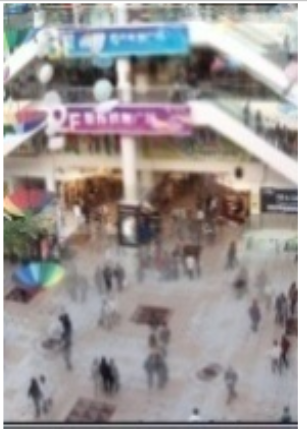
\includegraphics[scale=0.22]{images/feathering1}

\includegraphics[scale=0.24]{images/feathering2}
\caption{Feathering blending}
\label{fig:feathering}
\end{subfigure}
\begin{subfigure}[b]{0.495\textwidth}
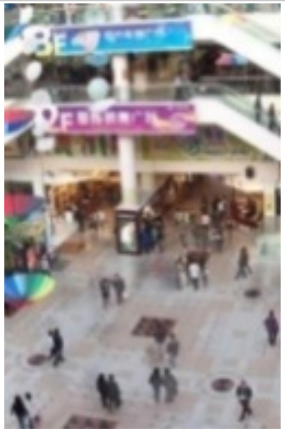
\includegraphics[scale=0.22]{images/multiband1}

\includegraphics[scale=0.24]{images/multiband2}
\caption{Muliband blending}
\label{fig:multiband}
\end{subfigure}
\caption{Examples of two different images blended using (a) feathering blending or (b) multiband blending. In the first case, the image preserves many people ghost images, and the text is blurred. Multiband blending produces an image with less people ghosting artifacts and with sharper text.}
\end{figure}





